\documentclass[12pt,letterpaper]{article}

\usepackage{amsmath}
\usepackage[pdftex]{graphicx}
\usepackage{hyperref} 

\parindent 0cm

\graphicspath{{figures/}}

\author{
    E. Jed Barlow\\
    \textit{ejbarlow@ualberta.ca}
}
\title{RpkmVisualizer Plugin Manual}

\begin{document}
\maketitle

\hfill

\tableofcontents

\newpage
\section{Overview}
RpkmVisualizer operates on the output of RNA-SEQ to generate a circular bar
graph of RPKM values for regions of a genome, or pan-genome.  The plugin is
meant to be used as part of gene abundance analysis of populations.

\section{Installation}
The plugin can be obtained, at the time of the writing of this manual, from two
locations.

\begin{itemize}
\item
    In source form: \url{http://github.com/jedbarlow/rpkmvisualizer}
\item
    As a compiled package: \url{http://www.ualberta.ca/~ejbarlow/biol498/}
\end{itemize}

Once obtained, the plugin \textit{rpkmvisualizer.cpa} can be installed as
follows.  First, click the \texttt{Plugins} in the CLC Genomics Workbench
toolbar in the top-right corner of the main window.

\begin{center}
    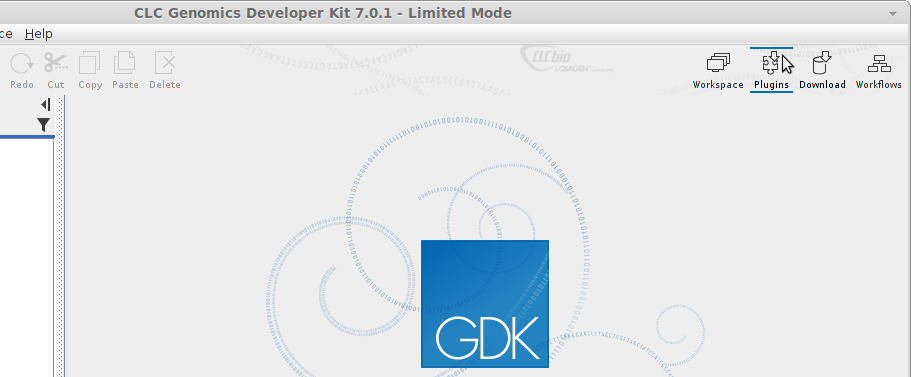
\includegraphics[width=34em]{plugins-button.png}
\end{center}

Then click the \texttt{Install From File} button.

\begin{center}
    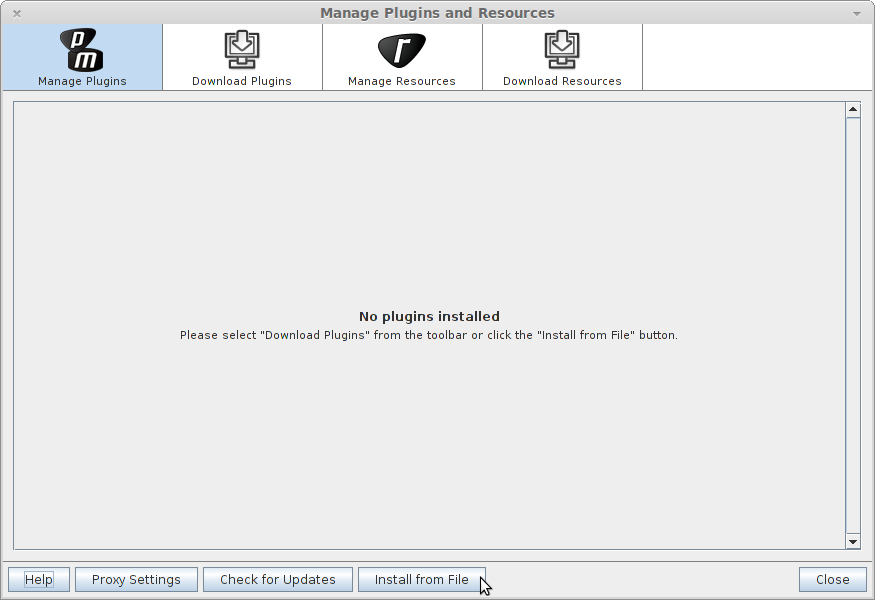
\includegraphics[width=34em]{install-from-file-button.png}
\end{center}

Then navigate to the folder containing the \texttt{rpkmvisualizer.cpa} file,
select the file, and click the \texttt{Install From File} button.

\begin{center}
    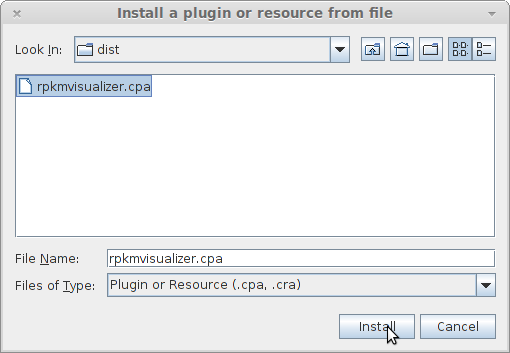
\includegraphics[width=26em]{install-button.png}
\end{center}

Then follow the on-screen steps of the wizard.  Once installed, an entry should
appear in the \texttt{Show} viewing option menu as shown in the figure in the
next section below.

\section{Operation}

In the CLC Genomics Workbench explorer pane, right-click on the result table of
the RNA-SEQ tool, and navigate to the \texttt{RPKM Heat Map} option as shown in
the following screenshot.

\begin{center}
    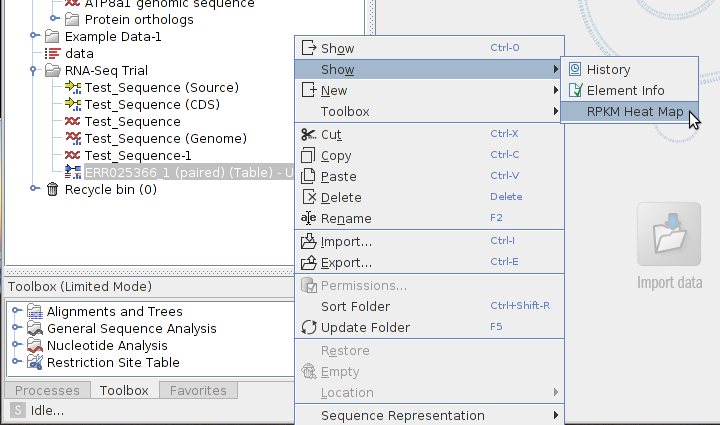
\includegraphics[width=34em]{access-plugin.png}
\end{center}

This will cause a view to be opened of the circular bar graph figure, similar
to the following example image.

\begin{center}
    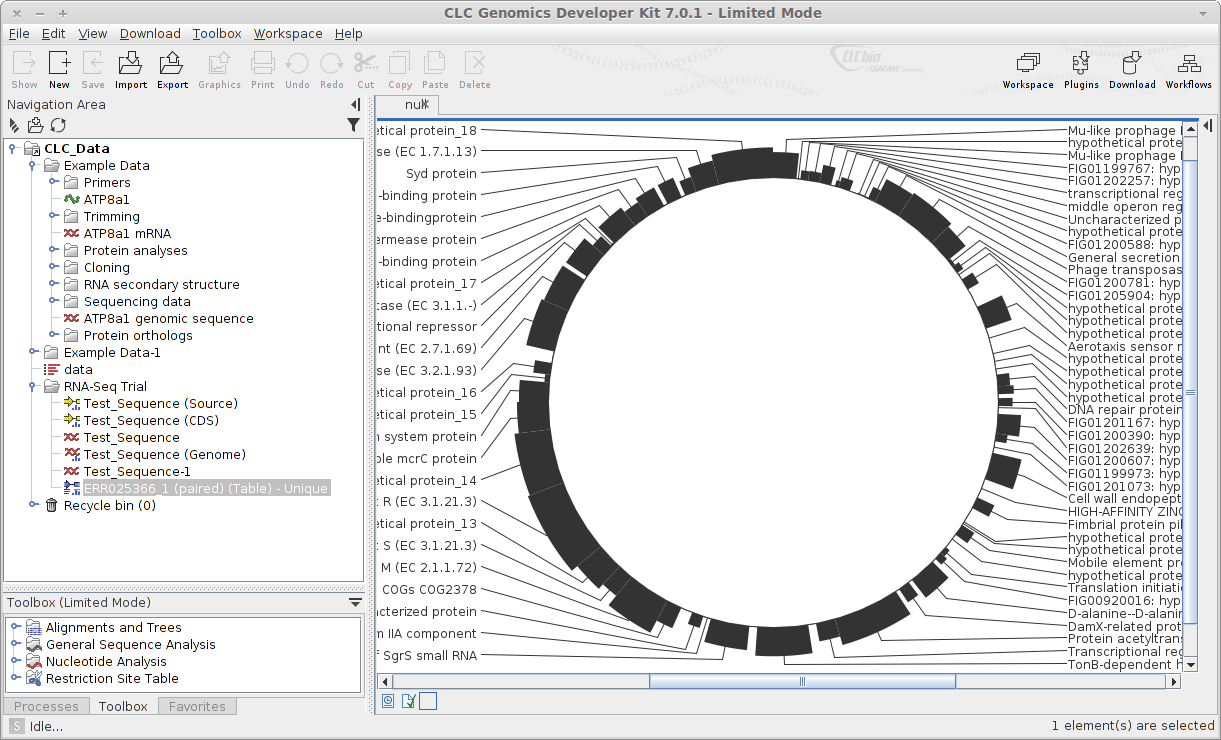
\includegraphics[width=32em]{plugin-result.png}
\end{center}

A sidebar with options can be accessed by clicking the arrow near the top-right
corner of the figure, next to the vertical scrollbar.

\begin{center}
    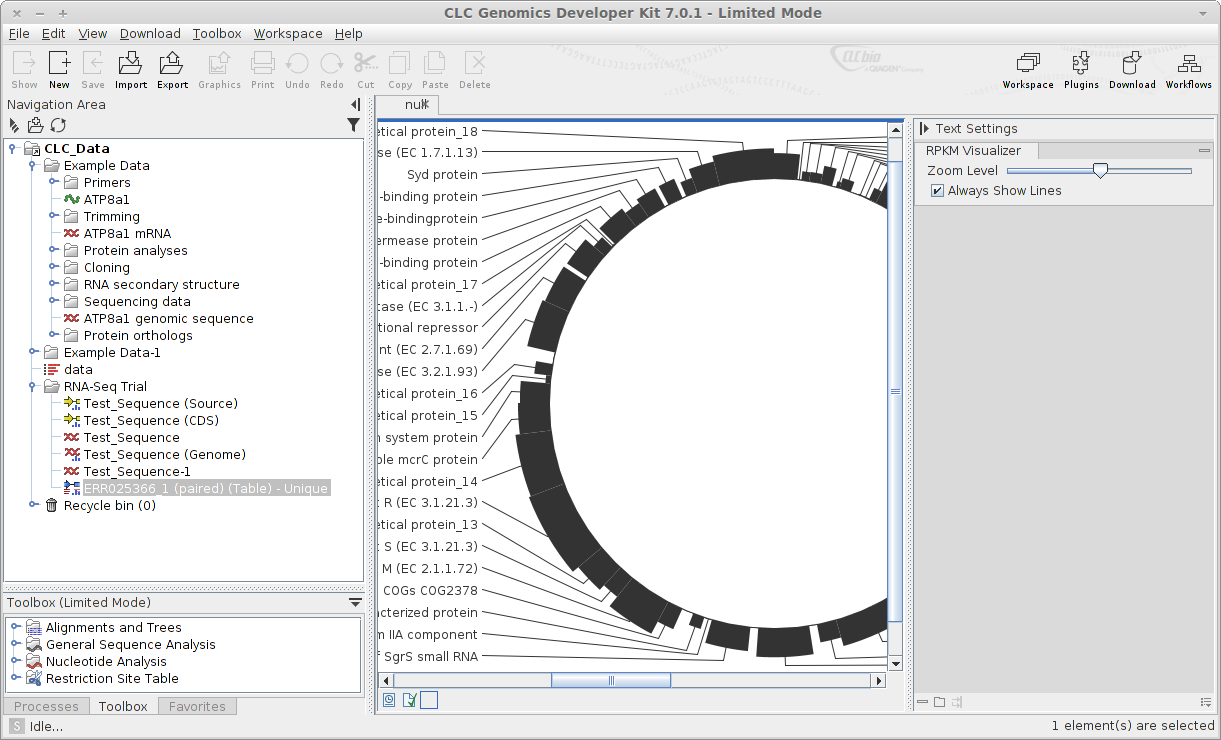
\includegraphics[width=32em]{sidebar.png}
\end{center}

These options can be used to adjust basic parameters of the figure, such as
zoom level and other layout options.

\begin{center}
    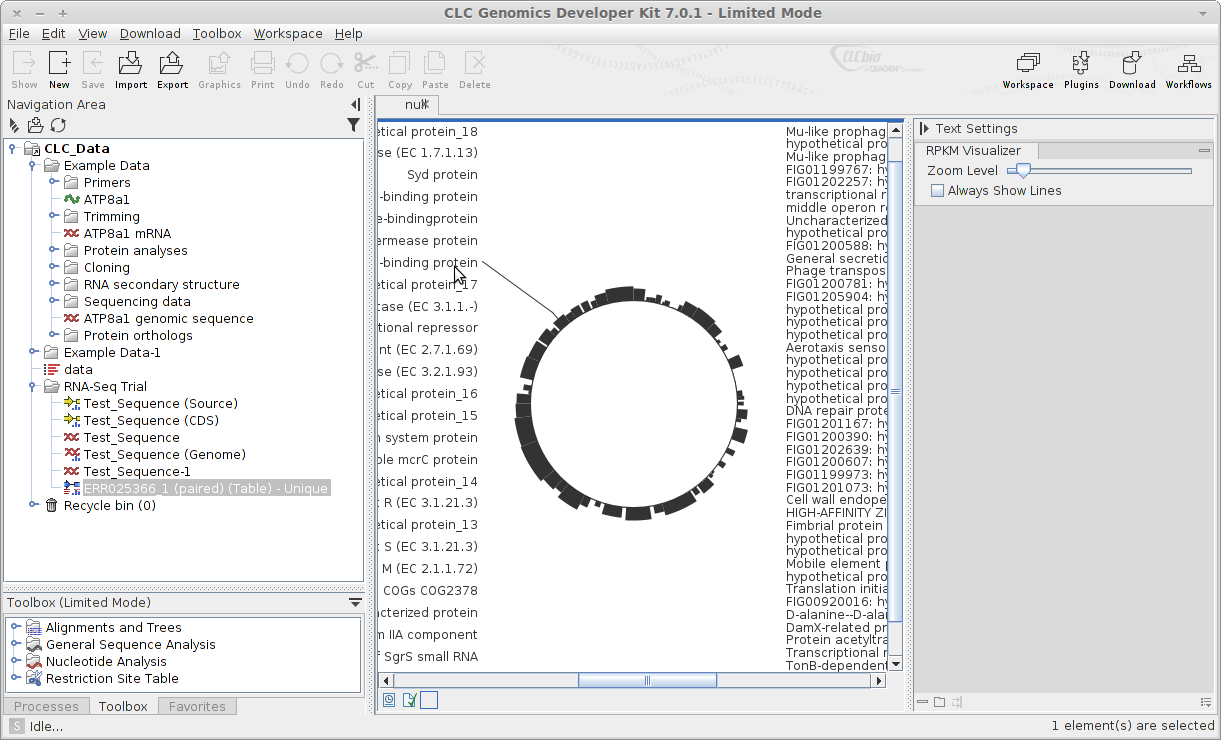
\includegraphics[width=32em]{sidebar-changed.png}
\end{center}

\end{document}
